\documentclass[11pt]{article}
\usepackage[margin=1in]{geometry}
\usepackage{graphicx}
\usepackage{amsmath}
\usepackage{amssymb}
\usepackage{booktabs}
\usepackage{placeins}
\usepackage[utf8]{inputenc}
\usepackage[T1]{fontenc}
\usepackage{xurl}
\usepackage{float}
\usepackage{titlesec}
\usepackage{authblk}
\titleformat{\section}{\large\bfseries}{\thesection}{0.6em}{}
\titleformat{\subsection}{\bfseries}{\thesubsection}{0.6em}{}
\hbadness=200
\vbadness=200
\hfuzz=2pt
\clubpenalty=10000
\widowpenalty=10000
\displaywidowpenalty=10000
\raggedbottom

\title{\large\bfseries Analyzing the Network of Disease Distribution by Country and Distance}
\author{Star A. Oje}
\affil{Department of Mathematics and Statistics, Washington State University}
\date{}

\begin{document}

\maketitle

\begin{abstract}
Infectious disease surveillance accumulates a large relational dataset: every reported
outbreak links a country to a disease and a year. This paper constructs a global network
from outbreak records spanning 233 countries and seventy diseases between 1996 and 2022 and
analyzes it along two complementary axes. The temporal axis tracks how centrality, the
influence and connectivity of individual countries, evolves year by year, revealing a
network that is structurally resilient (a maximum k-core of 221) but whose connectivity
surges sharply during major pandemics. The geospatial axis weights edges by geographic
proximity and tests directly whether distance shapes the resulting structure. A Mantel
permutation test, the appropriate tool for correlating two matrices defined over the same
set of nodes, shows that geographic distance is significantly associated with disease
co-reporting (Pearson $r=-0.192$, permutation $p<0.0001$ over 9{,}999 permutations), a
relationship that holds, and is in fact stronger, when the COVID-19 pandemic years are
included. Because geographically close countries are also often well connected by direct
flights, a partial Mantel test controlling for air-travel connectivity confirms the distance
effect survives, weakening only slightly (partial $r=-0.176$, $p<0.001$). Stratifying this
confound-controlled test by disease transmission mode shows the distance effect is weakest
for vector-borne disease and strongest for respiratory disease, a pattern consistent with
environmental filtering by global climate zone overriding simple geographic proximity for
vector-borne disease distribution. These results give the spatial intuition behind global
disease surveillance a quantitative foundation and identify Germany, Russia, and the small
island and territorial states of the Caribbean as structurally distinct types of nodes,
central hubs in one case, geographically isolated outliers in the other, that warrant
different surveillance strategies.
\end{abstract}

\noindent\textbf{Keywords:} network science, infectious disease, centrality, k-core
decomposition, Mantel test, partial Mantel test, geospatial analysis

\section{Introduction}

Infectious diseases continue to pose a global health challenge, causing widespread
morbidity and mortality despite advances in medical technology, vaccine development, and
public health awareness. Increasing global mobility and the resulting complexity of
interaction between populations make the spread of infectious disease harder to manage and
harder to anticipate \cite{baker2022}. This paper applies network science to the spread of
infectious disease across countries, explicitly incorporating geographic distance into the
analysis. Network science has already demonstrated its value in biology, neuroscience, and
health science more broadly \cite{barabasi2023,serban2020,leme2020}, and the same tools
transfer naturally to disease surveillance, where the relevant question is not just which
countries report a disease but how those countries are connected to one another through
shared outbreaks.

\subsection{Significance of the Study}

Infectious diseases remain among the ten leading causes of death worldwide
\cite{who2020}. Their persistent threat, combined with their capacity to spread rapidly
across borders, motivates analytical approaches that characterize disease dynamics at a
scale individual case reports cannot. Network science converts a large table of
country-disease-year records into a structure whose shape, which countries are central,
which are peripheral, which regions cluster together, can be read directly off the data.

This matters for two practical reasons beyond the descriptive value of the network itself.
International disease surveillance operates under fixed resources, and a tool that
identifies which countries function as structural bridges, rather than simply which
countries report the most cases, gives surveillance planners a way to prioritize monitoring
and response capacity toward locations whose loss would disconnect otherwise distant parts
of the network, not just locations with high case counts. Betweenness centrality and k-core
membership carry exactly this kind of structural signal, and neither is visible from
country-level case counts alone. The role geography plays in this structure is also
shifting: global air travel and mobility already reshape how diseases move between regions
relative to simple geographic distance \cite{balcan2009}, and climate change is expanding
the geographic range of vector habitats into regions that were not previously
climate-suitable \cite{paz2024}. Any distance-based account of disease structure measured
today is therefore a snapshot of a relationship likely to shift over time, and establishing
statistically how strongly geography currently predicts disease co-reporting, and whether
that relationship survives controlling for travel connectivity, provides a quantitative
baseline against which future shifts driven by mobility and climate change can be measured.

The network built here connects countries rather than individuals. An edge records that two
countries reported the same disease in the same year, a different claim from a confirmed
transmission event linking two specific cases. Person-to-person contact networks and
mobility-based transmission models operate at a finer resolution and answer a different
question: how a disease moves from one infected person to the next \cite{balcan2009}. The
country-level network instead serves disease surveillance at the resolution surveillance
data actually has available, standardized and openly reported across 233 countries and
seventy diseases simultaneously, a scale person-level contact-tracing data does not reach.
Section~\ref{sec:limitations} returns to this distinction in assessing what the results
below can and cannot support.

\subsection{Objectives}

The primary objective of this work is to construct and analyze a network model of
infectious disease spread between countries that accounts for the geographic distance
separating them. This makes it possible to identify which countries play disproportionate
roles in disease propagation, to track how those roles shift over time, and to test
directly whether geographic proximity makes disease co-reporting more likely. The result
informs disease surveillance and intervention strategy: knowing which countries function as
structural bridges, and whether that function depends on geography, has direct bearing on
where surveillance resources are likely to matter most.

\section{Related Work}

Network science has previously been applied to infectious disease outbreak patterns.
Torres Mungu\'{i}a et al.~\cite{torres2022}, whose dataset underlies this analysis,
characterized the spatial distribution of outbreak-prone diseases and identified clusters
of elevated susceptibility, establishing that geographic clustering exists in this dataset
without testing whether that clustering is attributable to distance itself or to a
correlated factor. Kim et al.~\cite{kim2021} used Monte Carlo simulation to assess epidemic
spread risk and concluded that reducing human contact is an effective lever for curbing
transmission, working from a contact-network framing rather than a country-level reporting
network. Neither study combines temporal centrality evolution with geospatial structure in
the same network, and neither subjects a distance-based hypothesis to a permutation test
capable of accounting for the non-independence of country-pair observations.

This paper advances that line of work in three respects. First, it tracks centrality and
k-core structure across the full 1996--2022 period rather than at a single cross-section,
revealing how connectivity responds to globally synchronized events such as the COVID-19
pandemic. Second, it replaces the qualitative observation that nearby countries report
diseases together more often with a Mantel permutation test, the correct tool given that
country-pair distances and co-reporting counts are not independent draws. Third, it tests
whether that distance effect is itself attributable to a known confound, air-travel
connectivity, using a partial Mantel test, and stratifies the result by disease transmission
mode, a level of statistical scrutiny not present in the descriptive network studies that
precede it.

\section{Problem Definition}

Identifying which countries occupy structurally central positions in a disease-reporting
network, and whether that structure is predictable from geography, has direct
consequences for surveillance design. A public health body deciding where to place
limited surveillance capacity, or which countries' reporting delays would propagate
furthest through the international system, needs to know whether central position is
stable over time or shifts with events such as a pandemic, and whether proximity to other
high-reporting countries is enough to predict a country's structural importance or
whether that relationship only holds once shared travel infrastructure is accounted for.
Neither question can be answered by the descriptive clustering result already
established in the literature reviewed above; both require treating centrality and
distance as quantities to be tracked over time and tested statistically, which motivates
the two questions this study addresses.

First, which countries played key structural roles in disease spread, and how has that
role changed over time? Second, does geographic distance shape the pattern of disease
co-reporting between countries, and can that relationship be established statistically
rather than observed only qualitatively, and does it survive once air-travel connectivity
is controlled for? Two analytical components address these questions in turn. Temporal
analysis constructs a time-sliced network for each year in the study period and tracks
how centrality measures evolve, revealing shifts in which countries occupy structurally
important positions as the network grows and changes. Geospatial analysis constructs a
weighted network in which edge weight reflects the physical distance between countries,
then tests whether that weighting predicts co-reporting behavior, first descriptively,
through clustering and spatial degree, and then statistically, through the permutation
tests developed in Section~\ref{sec:methodology}.

\section{Methodology}
\label{sec:methodology}

\subsection{Network Construction}

Two countries are connected by an edge if they have both reported the same disease in the
same year. An edge therefore captures shared exposure to a reporting event; it does not
claim that the disease was transmitted directly between the two countries, since the
dataset records outbreak occurrence, not transmission pathways. For temporal analysis, the
network is sliced into one graph per year. For the aggregate analyses in
Section~\ref{sec:results}, edges accumulate weight equal to the number of distinct
disease-year combinations the two countries share, so that countries with a long history of
overlapping outbreaks are more strongly connected than countries that happened to share a
single event.

\subsection{Centrality Measures}

Four centrality measures characterize node importance, each capturing a different aspect of
a country's position in the network. Degree centrality counts a country's direct
connections, weighted by connection strength in the weighted network, and reflects how
broadly a country's reported diseases overlap with other countries' reported diseases.
Betweenness centrality counts how often a country lies on the shortest path between two
other countries; a country with high betweenness functions as a structural bridge, since
removing it would lengthen the path between many pairs of other countries, corresponding in
the disease context to a potential bottleneck or conduit for transmission. Closeness
centrality measures how few steps separate a country from every other country in the
network, with high closeness indicating a country positioned to reach, or be reached by,
the rest of the network quickly. Eigenvector centrality weights a country's connections by
the importance of the countries it is connected to, so that a link to a highly central
country contributes more than a link to a peripheral one, identifying countries that are
influential by virtue of who their connections are with, not just how many they have.

This project emphasizes degree and betweenness centrality in the year-by-year analysis of
Section~\ref{sec:temporal}, since they map most directly onto the questions of connectivity
and critical transmission pathways that motivate this study; closeness and eigenvector
centrality are reported for completeness and discussed where they diverge informatively
from the first two.

\subsection{K-core Decomposition}

K-core decomposition simplifies a network by iteratively removing nodes with fewer than $k$
connections, peeling away the periphery to reveal the most densely interconnected core. The
resulting core number for each node indicates how deeply embedded that node is in the
network's most connected substructure, and the maximum core number across the network
summarizes how resilient the network's core is to the loss of individual nodes
\cite{montresor2012}.

\subsection{Statistical Validation Framework}

Section~\ref{sec:results} produces descriptive impressions: that connectivity surges during
pandemics, that the network has a deeply interconnected core, that nearby countries seem
more strongly linked. The third of these, the relationship between geographic distance and
co-reporting strength, is directly testable using a Mantel test \cite{mantel1967}.

The Mantel test is the appropriate tool because the two quantities being compared, the
matrix of pairwise geographic distances and the matrix of pairwise co-reporting strengths,
are both defined over the same 233 countries. A standard correlation test assumes
independent observations, but every entry in a distance matrix shares a row or column with
every other entry involving the same country, so the $\binom{233}{2}$ country pairs are not
independent draws. The Mantel test builds an empirical null by repeatedly permuting the row
and column labels of one matrix, which preserves each matrix's internal structure while
breaking any underlying association between the two, and asks how extreme the observed
correlation is relative to that empirical null. We compute the Pearson correlation between
the upper-triangular entries of the two matrices, generate a null distribution from 9{,}999
label permutations, and report the resulting two-sided permutation $p$-value. A Spearman
version is also reported as a check against a relationship that is monotonic but not
linear.

A significant Mantel correlation does not rule out that distance and co-reporting are both
driven by a third factor. Countries that are geographically close are also often well
connected by direct flights, and flight connectivity is plausibly tied to shared trade,
tourism, and surveillance-reporting practices that could independently produce correlated
reporting behavior. We extend the test to a partial Mantel test \cite{smouse1986}, which
asks whether distance and co-reporting remain correlated once their shared association with
a third matrix, here a country-pair air-travel connectivity matrix built from flight route
data, is removed. The partial correlation is
\begin{equation}
r_{XY \cdot Z} = \frac{r_{XY} - r_{XZ}\,r_{YZ}}{\sqrt{(1-r_{XZ}^2)(1-r_{YZ}^2)}}
\label{eq:partial}
\end{equation}
where $X$, $Y$, and $Z$ are the vectorized upper-triangular entries of the distance,
co-reporting, and connectivity matrices, respectively. Significance is assessed by
permuting the row and column labels of the distance matrix $X$ only, holding $Y$ and $Z$
fixed, and recomputing the partial correlation at each of 1{,}999 permutations, the scheme
recommended for partial Mantel tests because permuting $X$ alone tests whether the $X$-$Y$
relationship persists beyond what $X$ shares with $Z$, without disturbing the underlying
$Y$-$Z$ relationship being controlled for \cite{legendre2000}. We additionally repeat this
partial Mantel procedure within three disease transmission-mode strata, vector-borne,
respiratory, and waterborne/foodborne (Section~\ref{sec:connectivity-data}), to test whether
the distance effect net of travel connectivity differs by how a disease spreads.

\FloatBarrier

\section{Data}

\subsection{Dataset Description}

Two datasets support this analysis. The first, sourced from Torres Mungu\'{i}a et
al.~\cite{torres2022}, records seventy distinct infectious diseases reported across 233
countries from January 1996 to March 2022, where a unique outbreak is defined as at least
one reported case of a specific disease in a given country within a given year. The second
provides latitude and longitude for 245 countries \cite{metal3d2024}; pairwise distances are
computed with the Haversine formula, which gives the great-circle distance between two
points on the Earth's surface from their coordinates, assuming an Earth radius of 6{,}371
kilometers \cite{haversine2024}. This distance convention is consistent with standard
practice in the gravity-model literature on geographic distance, including the GeoDist
database \cite{mayer2011}.

\subsection{Exploratory Data Analysis and Network Construction}

Exploratory analysis identified and removed six duplicate entries for one country spanning
2020 to 2022, leaving 2{,}221 entries. Table~\ref{tab:diseases} summarizes the ten most
frequently reported diseases over the study period; COVID-19 and influenza dominate by a
wide margin, each reported far more often than the next most common disease, cholera.
Fig.~\ref{fig:worldmap} maps the total number of unique diseases reported by each country
across the full study period, showing the United States, China, and several Western
European countries reporting the broadest diversity of diseases, a pattern that likely
reflects surveillance capacity as much as underlying disease burden.

\begin{table}[H]
\centering
\caption{Ten Most Frequently Reported Diseases, 1996--2022}
\label{tab:diseases}
\begin{tabular}{lc}
\toprule
Disease & Count \\
\midrule
COVID-19 & 659 \\
Influenza & 409 \\
Cholera & 112 \\
Acute Poliomyelitis & 112 \\
Yellow Fever & 104 \\
Meningitis & 95 \\
Measles & 83 \\
MERS & 67 \\
Dengue & 50 \\
Viral Haemorrhagic Fever & 49 \\
\bottomrule
\end{tabular}
\end{table}

\begin{figure}[H]
\centering
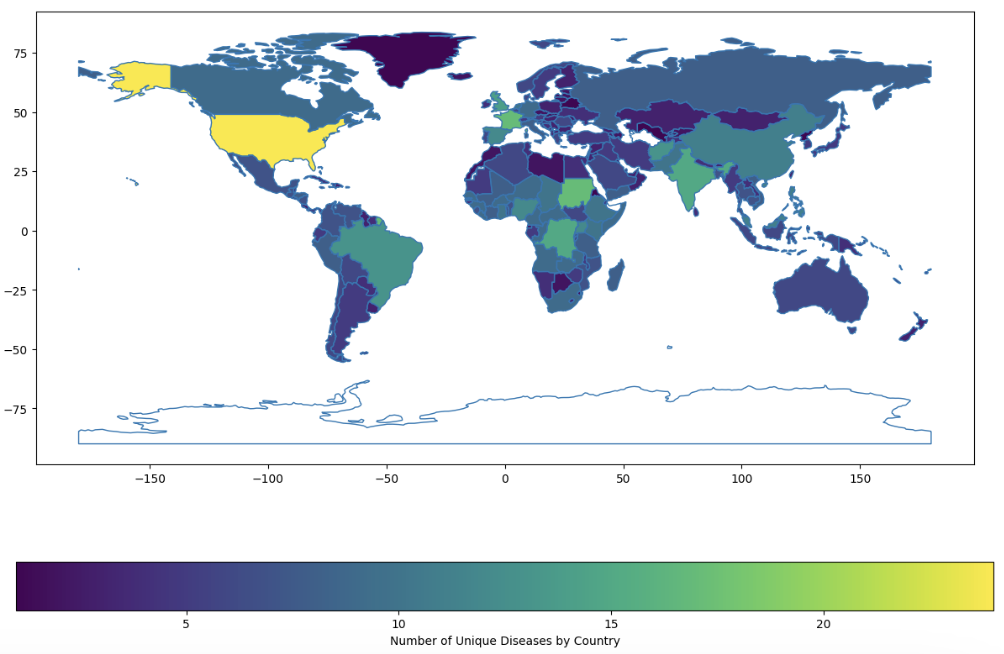
\includegraphics[width=0.85\linewidth]{figures/world_map_unique_diseases.png}
\caption{Total number of unique diseases reported by each country, 1996--2022.}
\label{fig:worldmap}
\end{figure}

The resulting aggregate network comprises 233 nodes and 26{,}203 edges, with the disease and
year of each shared report stored as edge attributes. The top countries by degree and
closeness centrality are the United States, China, France, and Germany, with many other
countries tied at the same values; the top countries by betweenness centrality are Germany,
Russia, Sudan, the Democratic Republic of the Congo, and the Republic of the Congo. These
two rankings already hint at the distinction developed further below: degree and closeness
identify countries with broad diagnostic and reporting capacity, while betweenness
identifies countries whose position in the network makes them structural bridges
regardless of their own report volume.

\FloatBarrier

\subsection{Connectivity and Disease Transmission-Mode Data}
\label{sec:connectivity-data}

The partial Mantel test in Section~\ref{sec:methodology} requires a third matrix: a measure
of direct air-travel connectivity between each pair of countries, independent of
co-reporting. We build this from OpenFlights' public airport and route data
\cite{openflights2024}, mapping each route's source and destination airports to a country
and counting the number of distinct scheduled routes connecting each pair of countries,
summed over both directions. This is a coarse proxy: it counts route legs, not passenger
volume, and 1{,}078 of 67{,}663 routes (1.6 percent) could not be resolved to a country
because of naming mismatches between the airport records and the outbreak dataset's country
codes and were dropped rather than guessed. Of the $\binom{233}{2}=27{,}028$ country pairs
in the network, 2{,}271 have at least one direct route, a sparsity consistent with the
hub-and-spoke structure of real global aviation networks.

Disease transmission mode is assigned per disease from CDC and WHO disease-page
descriptions of how each pathogen is primarily transmitted, sorting the seventy diseases in
the dataset into vector-borne (nineteen diseases, including malaria, dengue, and yellow
fever), respiratory (eleven diseases, including influenza, COVID-19, and measles), and
waterborne/foodborne (thirteen diseases, including cholera, typhoid, and acute
poliomyelitis). Fourteen diseases with a known but different transmission route (direct
contact, bloodborne, or zoonotic-environmental, including Ebola, HIV, and rabies) are
retained as a labeled but separate category and excluded from the three-way stratified test
since they do not share a common transmission mechanism with each other. Thirteen diseases
recorded with an unspecified causative agent, or that are not conventionally transmissible
person-to-person at all (for example Creutzfeldt-Jakob disease), are left unclassified
rather than assigned a route the data cannot support.

\FloatBarrier

\section{Results and Discussion}
\label{sec:results}

\subsection{Temporal Analysis}
\label{sec:temporal}

Constructing a separate network for each year and tracking average centrality over time
reveals two sharp departures from an otherwise noisy baseline: a peak around 2010 and a
sustained surge from 2020 through 2022.

\begin{figure}[H]
\centering
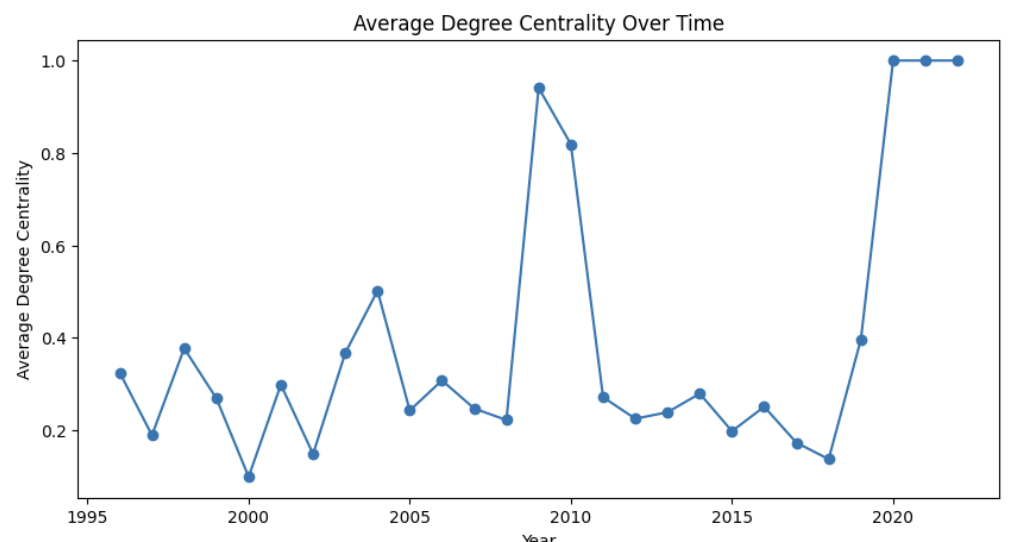
\includegraphics[width=0.48\linewidth]{figures/degree_centrality_time.png}
\hfill
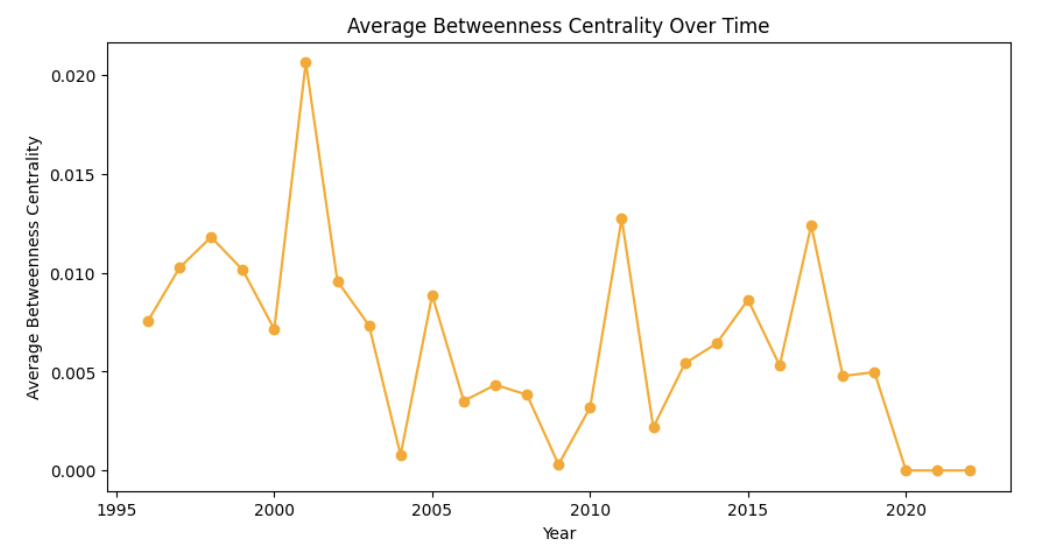
\includegraphics[width=0.48\linewidth]{figures/betweenness_centrality_time.png}
\caption{Average degree centrality (left) and average betweenness centrality (right) over
time.}
\label{fig:degree-betweenness}
\end{figure}

Fig.~\ref{fig:degree-betweenness} (left) shows average degree centrality rising and falling
between 1996 and 2019 without a clear trend, then jumping sharply in 2020. This jump
corresponds directly to COVID-19, which was reported by nearly every country in the network
within the same year, mechanically inflating connectivity because the network construction
in Section~\ref{sec:methodology} links any two countries that share a reported disease in a
given year.

Average betweenness centrality (Fig.~\ref{fig:degree-betweenness}, right) tells a different
story. Despite the connectivity surge of 2020--2022, betweenness centrality falls to nearly
zero in those years. When almost every country is connected to almost every other country
through the same globally reported disease, no single country acts as a bridge, since most
pairs of countries are already directly connected. The peak in 2001, by contrast, indicates
a year in which disease spread more through indirect chains, where certain countries
mediated the connection between others. This contrast between degree and betweenness during
the pandemic years illustrates a general property of network structure: a network can
become highly connected without becoming more dependent on any particular node, and the two
centrality measures together distinguish those situations in a way that degree alone
cannot.

\begin{figure}[H]
\centering
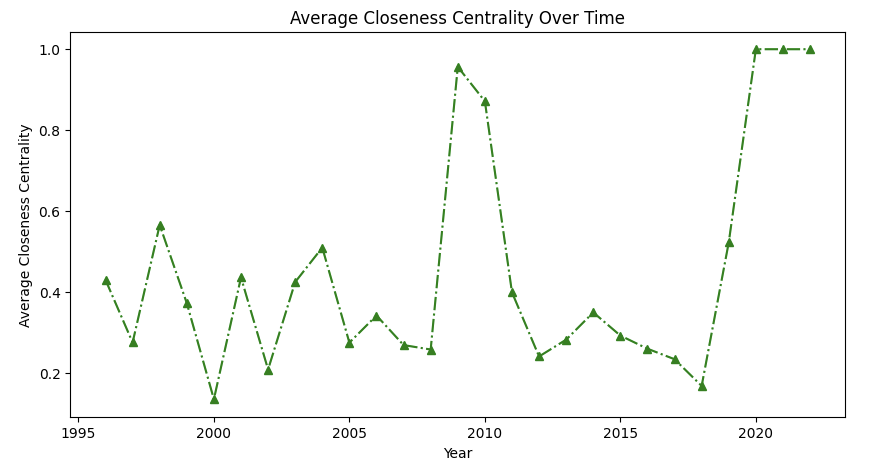
\includegraphics[width=0.48\linewidth]{figures/closeness_centrality_time.png}
\hfill
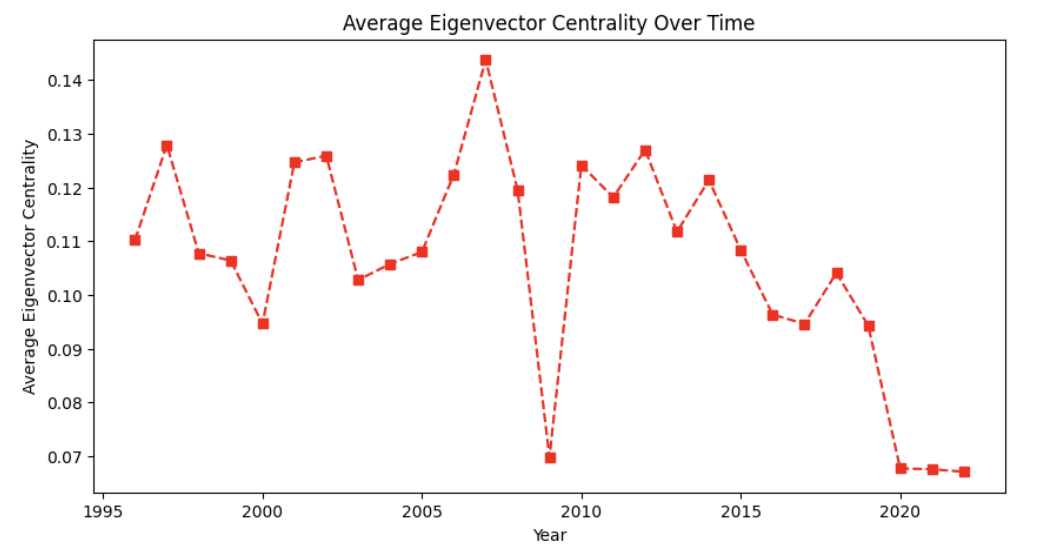
\includegraphics[width=0.48\linewidth]{figures/eigenvector_centrality_time.png}
\caption{Average closeness centrality (left) and average eigenvector centrality (right) over
time.}
\label{fig:closeness-eigenvector}
\end{figure}

Closeness centrality (Fig.~\ref{fig:closeness-eigenvector}, left) follows degree
centrality's pattern, rising sharply during 2009--2010 and again in 2020--2022, consistent
with a network in which most countries are within one or two steps of each other during
high-connectivity years. Eigenvector centrality (Fig.~\ref{fig:closeness-eigenvector},
right) moves in the opposite direction during the pandemic years, falling to its lowest
values in the study period. Eigenvector centrality rewards connections to already-important
countries, and when connectivity becomes nearly uniform across the entire network, the
distinction between connecting to an important country and connecting to any country
disappears, compressing the eigenvector centrality distribution toward uniformity.

\begin{figure}[H]
\centering
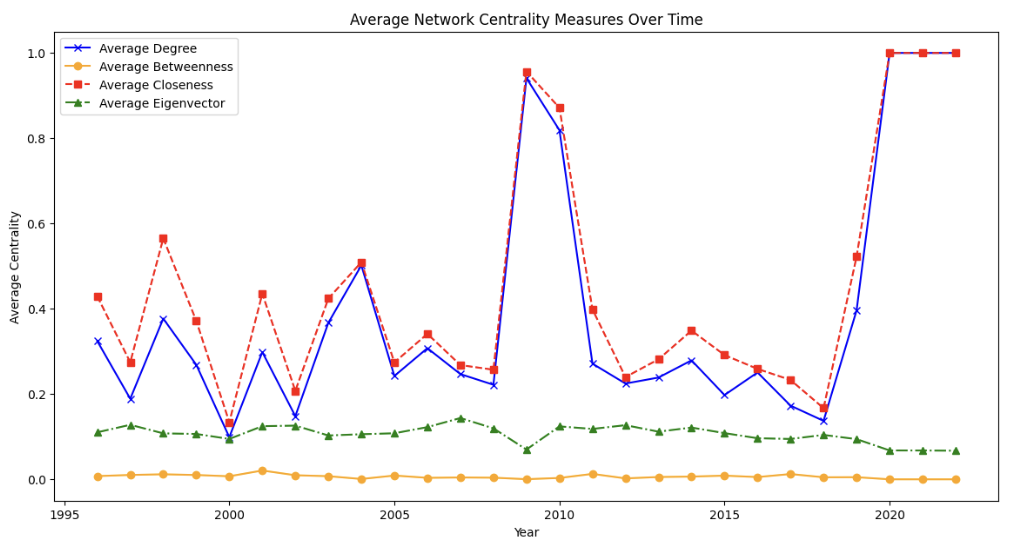
\includegraphics[width=0.65\linewidth]{figures/centrality_comparison_time.png}
\caption{All four average centrality measures over time, shown together.}
\label{fig:centrality-comparison}
\end{figure}

Fig.~\ref{fig:centrality-comparison} places all four measures on the same axes. Degree and
closeness move together throughout the study period, while betweenness and eigenvector
centrality stay low and comparatively flat, with eigenvector centrality declining further
still during the pandemic years. The overall picture is a network whose connectivity is
widespread rather than concentrated in a small set of hub countries, a structural property
the k-core analysis below examines more directly.

\FloatBarrier

Tracking degree centrality for a fixed set of countries across different regions, the
United States, Brazil, Australia, Colombia, China, Sudan, and Russia, shows substantial
heterogeneity that the global averages above obscure.

\begin{figure}[H]
\centering
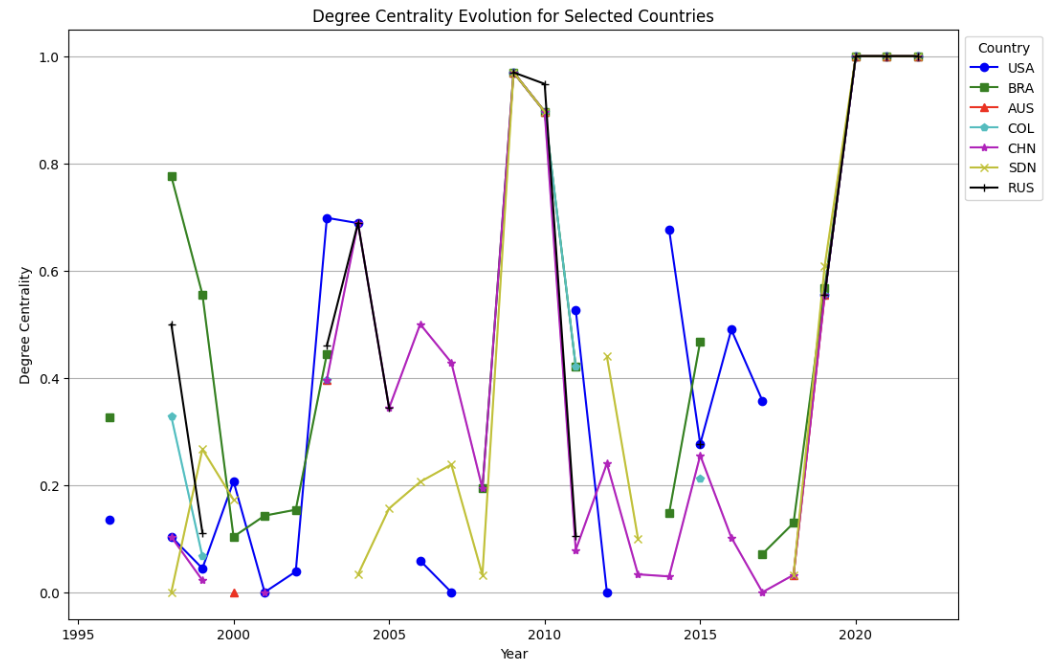
\includegraphics[width=0.7\linewidth]{figures/selected_countries_gaps.png}
\caption{Degree centrality evolution for selected countries, with years of no reported
disease left as gaps.}
\label{fig:selected-gaps}
\end{figure}

\begin{figure}[H]
\centering
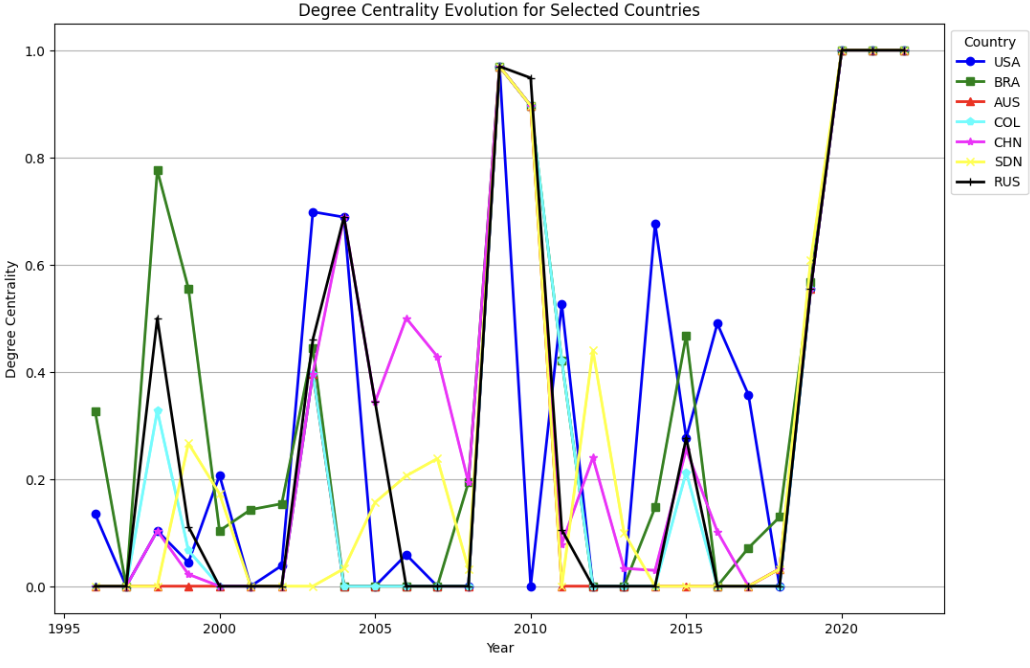
\includegraphics[width=0.7\linewidth]{figures/selected_countries_zero.png}
\caption{Degree centrality evolution for selected countries, with years of no reported
disease set to zero.}
\label{fig:selected-zero}
\end{figure}

These two treatments of missing reports answer different questions. The gap version
(Fig.~\ref{fig:selected-gaps}) shows each country's centrality conditional on having
reported at least one disease that year, while the zero-filled version
(Fig.~\ref{fig:selected-zero}) shows centrality unconditionally, including years of apparent
inactivity. The difference between the two figures measures how much a country's centrality
trajectory is driven by gaps in reporting rather than by an actual absence of disease
activity, a distinction that matters for interpreting any single country's trajectory.

\FloatBarrier

Because the average centrality measures above peak sharply around 2010, we examine
2008--2010 in more detail by constructing the network for each of those years individually.

\begin{figure}[H]
\centering
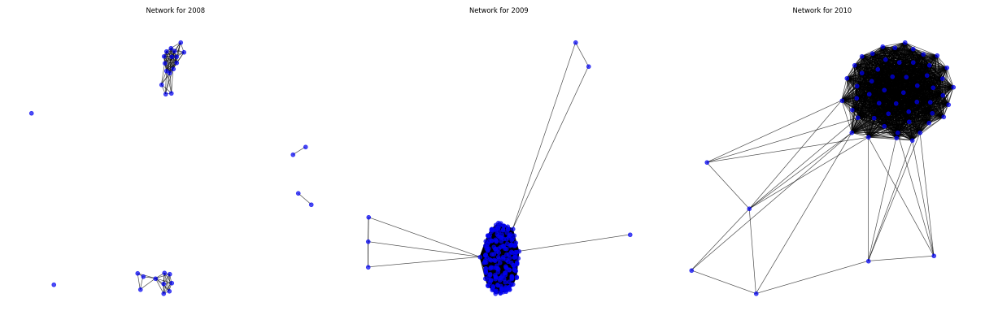
\includegraphics[width=0.85\linewidth]{figures/network_evolution_2008_2010.png}
\caption{Network structure in 2008, 2009, and 2010, showing the rapid densification of the
disease-reporting network over three years.}
\label{fig:evolution}
\end{figure}

Fig.~\ref{fig:evolution} shows isolated clusters in 2008 consolidating into a single dense
core by 2010. The disease driving this consolidation can be identified by decomposing the
2010 network into subgraphs for each individual disease reported that year.

\begin{figure}[H]
\centering
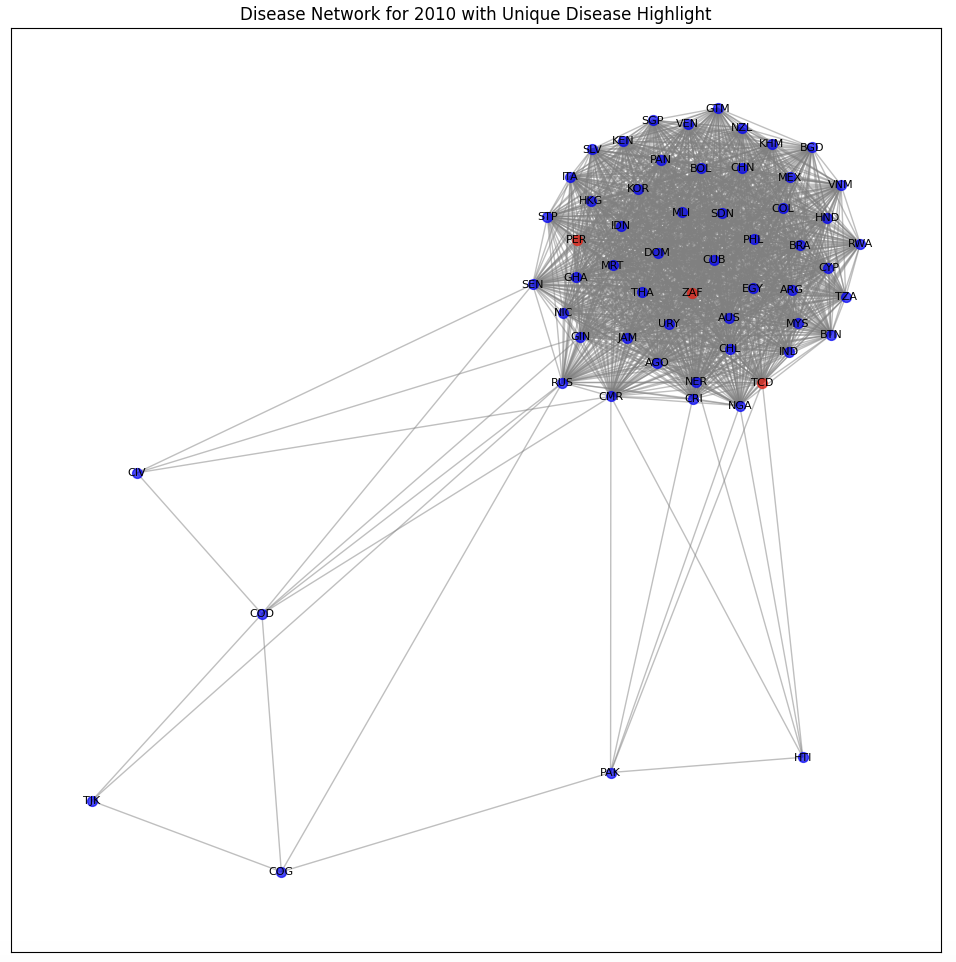
\includegraphics[width=0.55\linewidth]{figures/disease_network_2010_highlighted.png}
\caption{The full 2010 disease-reporting network, with countries that reported an
otherwise-isolated disease case highlighted.}
\label{fig:network2010}
\end{figure}

\begin{figure}[H]
\centering
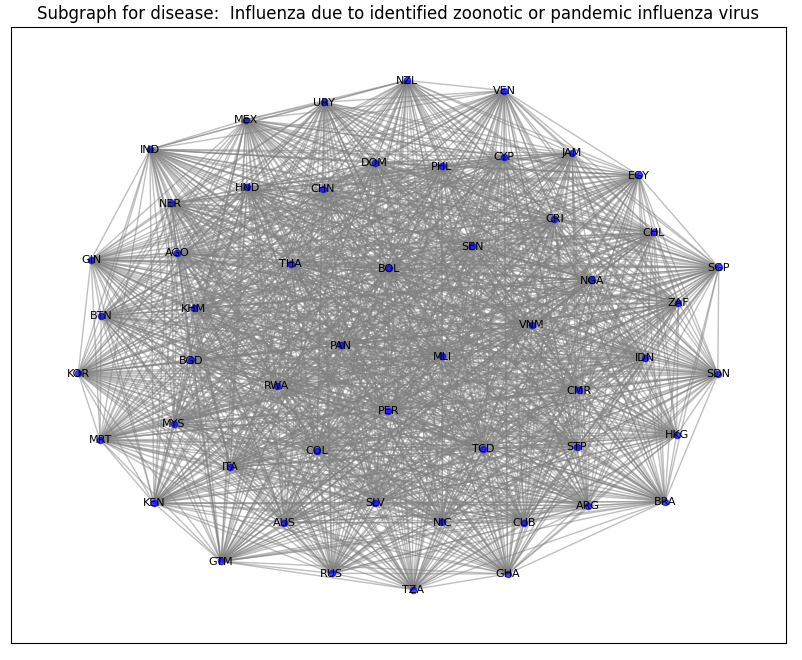
\includegraphics[width=0.48\linewidth]{figures/subgraph_influenza.png}
\hfill
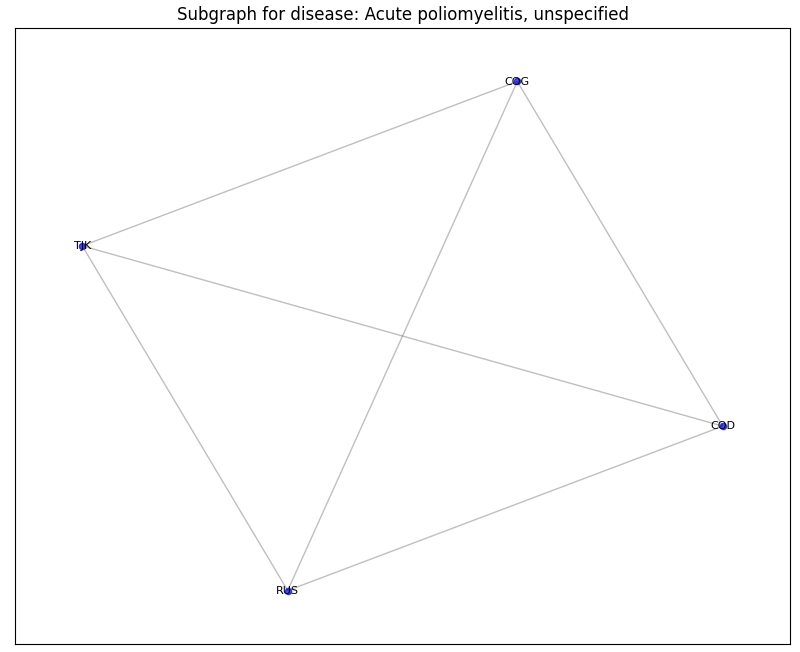
\includegraphics[width=0.48\linewidth]{figures/subgraph_polio.png}
\caption{Subgraphs for two diseases reported in 2010: influenza (left), forming a
near-complete graph among dozens of countries, and acute poliomyelitis (right), connecting
only four. The contrast illustrates how disease-specific reporting patterns range from
globally synchronized to highly localized within the same network and the same year.}
\label{fig:subgraphs}
\end{figure}

\FloatBarrier

To assess the network's resilience to the loss of individual nodes, we aggregate disease
reports across all years into a single weighted network, with edge weight equal to the
cumulative number of shared disease-year reports between each pair of countries, and apply
k-core decomposition.

\begin{figure}[H]
\centering
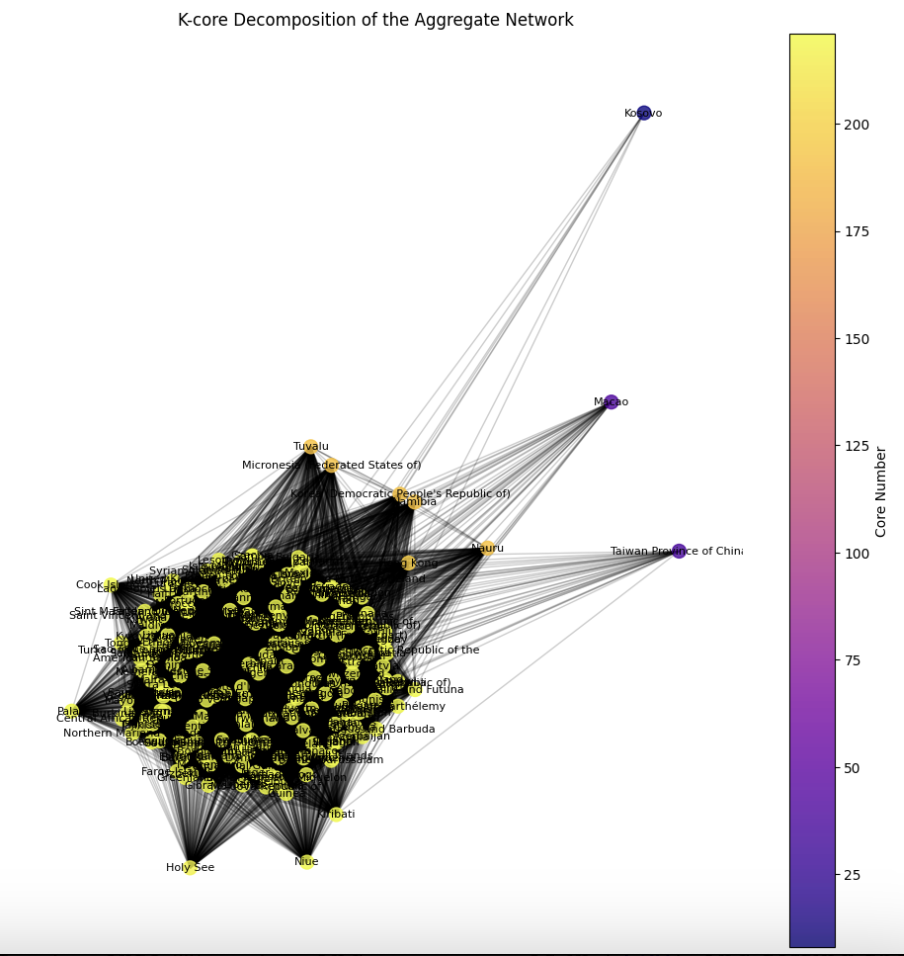
\includegraphics[width=0.6\linewidth]{figures/kcore_decomposition.png}
\caption{K-core decomposition of the aggregate network. Color indicates each node's core
number.}
\label{fig:kcore}
\end{figure}

The maximum core number is 221, and the great majority of nodes share this value, indicating
a network whose core is deeply and almost uniformly interconnected rather than concentrated
around a small set of hubs, consistent with the pattern already visible above: the
network's high connectivity is broadly distributed, not centrally coordinated.
Table~\ref{tab:centrality} reports centrality scores for a sample of nodes at the top and
bottom of the distribution. Canada, China, Hong Kong, Iran, and Israel sit at or near the
top by degree and closeness centrality, while Taiwan, Macau, and Kosovo sit near the
bottom, with Kosovo's degree centrality more than an order of magnitude lower than the
network median. These low values reflect each territory's limited diplomatic and reporting
infrastructure within the WHO surveillance system rather than an absence of disease
activity, an important caveat for interpreting any centrality ranking built from
international reporting data.

\begin{table}[H]
\centering
\caption{Centrality Scores for Selected High- and Low-Centrality Nodes}
\label{tab:centrality}
\begin{tabular}{lccc}
\toprule
Country & Degree & Betweenness & Closeness \\
\midrule
Canada (CAN) & 0.9914 & 2.38e-04 & 0.9915 \\
China (CHN) & 0.9957 & 4.14e-04 & 0.9957 \\
Hong Kong (HKG) & 0.8836 & 3.31e-04 & 0.8958 \\
Iran (IRN) & 0.9871 & 4.30e-05 & 0.9872 \\
Israel (ISR) & 0.9914 & 2.16e-04 & 0.9915 \\
Palau (PLW) & 0.9569 & 1.69e-07 & 0.9587 \\
Niue (NIU) & 0.9526 & 0.0000 & 0.9547 \\
Taiwan (TWN) & 0.1595 & 0.0000 & 0.5433 \\
Macau (MAC) & 0.1767 & 0.0000 & 0.5485 \\
Kosovo (XXK) & 0.0345 & 0.0000 & 0.5088 \\
\bottomrule
\end{tabular}
\end{table}

\FloatBarrier

\subsection{Geospatial Analysis}

This section integrates geographic distance directly into the network by weighting each
edge according to the distance between the two countries it connects, with weight defined
as the inverse of distance so that closer countries receive higher weight.

\begin{figure}[H]
\centering
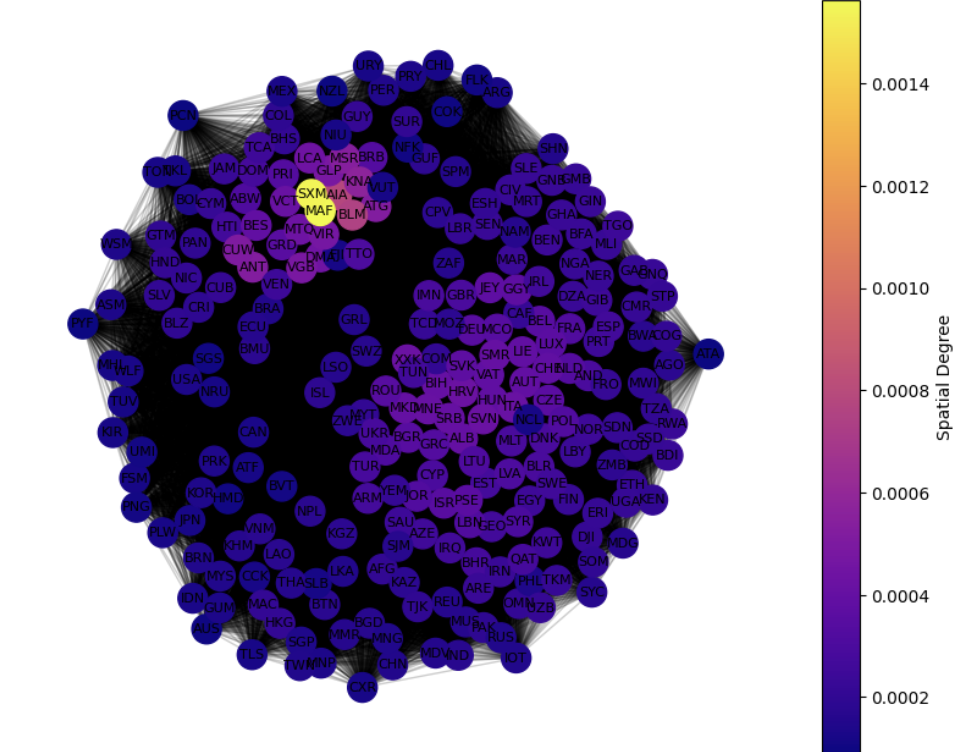
\includegraphics[width=0.4\linewidth]{figures/spatial_degree_network.png}
\caption{Network visualization colored by spatial degree, the average connection strength
of each node to its geographic neighbors.}
\label{fig:spatial-degree}
\end{figure}

Table~\ref{tab:strength} lists the five countries with the highest average connection
strength to their geographic neighbors. All five are small Caribbean island territories,
Saint Martin, Sint Maarten, Anguilla, Saint Barth\'{e}lemy, and Saint Kitts and Nevis, whose
high spatial degree reflects geographic proximity to a cluster of similarly small
neighboring territories rather than any particular disease burden.

\begin{table}[H]
\centering
\caption{Top Five Countries by Geographic Connection Strength}
\label{tab:strength}
\begin{tabular}{lc}
\toprule
Country & Strength \\
\midrule
Saint Martin & 0.389 \\
Sint Maarten & 0.386 \\
Anguilla & 0.193 \\
Saint Barth\'{e}lemy & 0.187 \\
Saint Kitts and Nevis & 0.142 \\
\bottomrule
\end{tabular}
\end{table}

\FloatBarrier

The weighted clustering coefficient measures how interconnected a node's neighbors are with
each other, identifying tightly-knit regional clusters.

\begin{figure}[H]
\centering
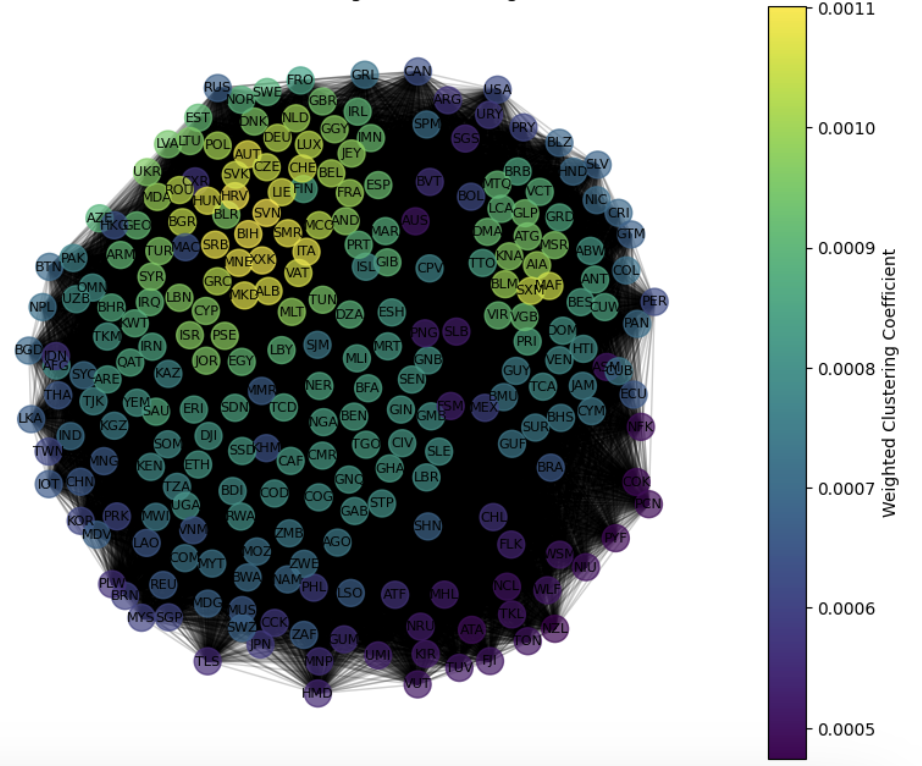
\includegraphics[width=0.4\linewidth]{figures/weighted_clustering_network.png}
\caption{Network visualization colored by weighted clustering coefficient.}
\label{fig:weighted-clustering}
\end{figure}

\begin{figure}[H]
\centering
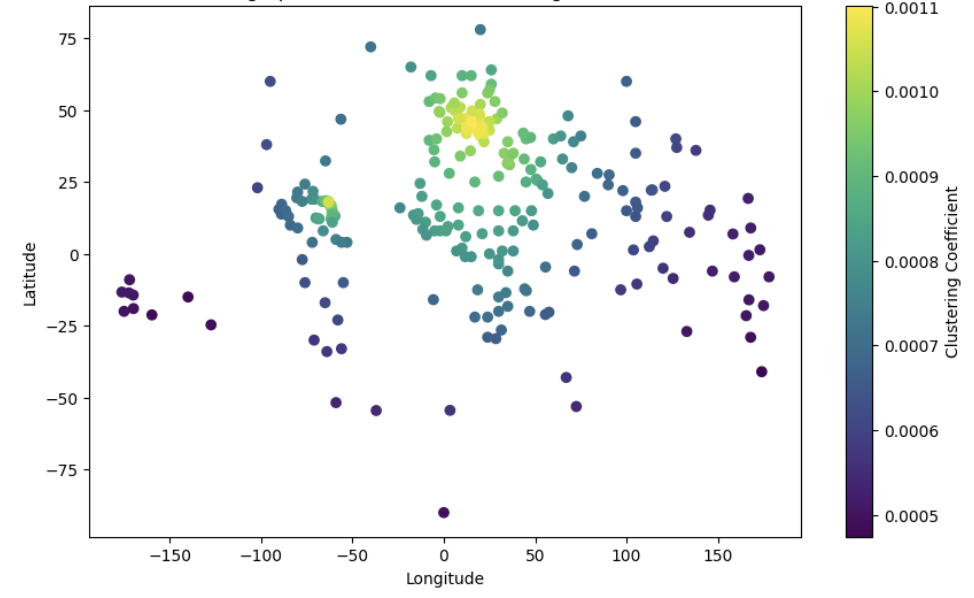
\includegraphics[width=0.65\linewidth]{figures/clustering_geographic_distribution.png}
\caption{Weighted clustering coefficients mapped onto geographic coordinates.}
\label{fig:clustering-map}
\end{figure}

Mapping the clustering coefficient onto each country's actual location
(Fig.~\ref{fig:clustering-map}) shows the highest values concentrated in Western and Central
Europe and in the Caribbean, both regions of small countries packed closely together, and
the lowest values among isolated Pacific island nations. This geographic concentration of
high clustering coefficients is the descriptive observation tested statistically below.

\begin{figure}[H]
\centering
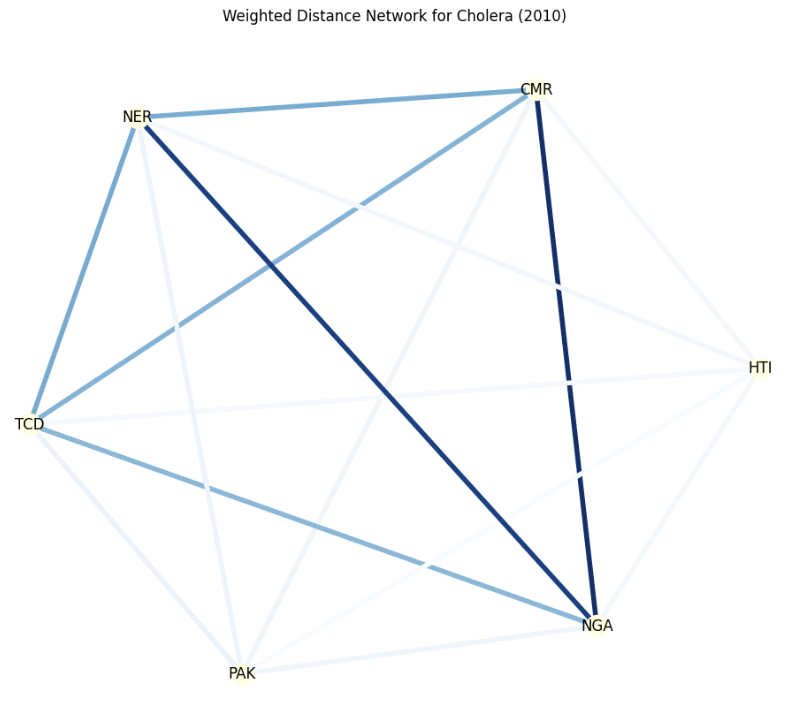
\includegraphics[width=0.48\linewidth]{figures/weighted_distance_cholera.png}
\hfill
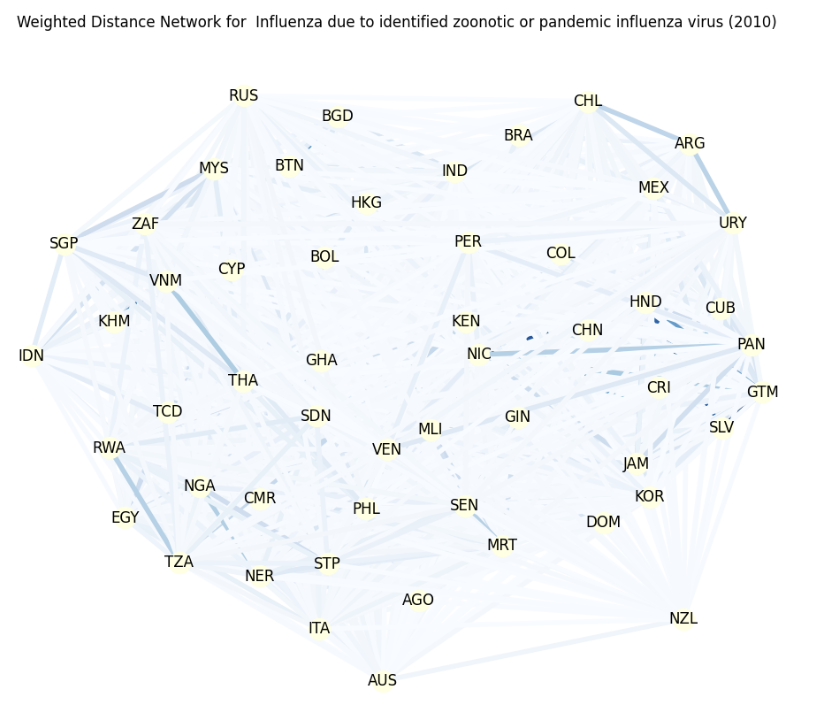
\includegraphics[width=0.48\linewidth]{figures/weighted_distance_influenza.png}
\caption{Weighted distance subgraphs for cholera (left) and influenza (right) in 2010.
Darker edges indicate shorter distances. Cholera's 2010 reports connect a small,
geographically dispersed set of countries with no consistent proximity pattern, while
influenza's far larger and more globally distributed 2010 reports show the weighted network
at a scale where any individual proximity relationship is visually difficult to assess,
motivating the network-wide statistical test below rather than visual inspection of
individual disease subgraphs.}
\label{fig:weighted-distance}
\end{figure}

\FloatBarrier

\subsection{Statistical Validation of the Distance Effect}

The clustering map in Fig.~\ref{fig:clustering-map} and the connection-strength results
above are consistent with geographic proximity shaping disease co-reporting, but
consistency is not confirmation. Applying the Mantel test from
Section~\ref{sec:methodology} to the full 1996--2022 network, restricted to the 233
countries with both outbreak and coordinate data, gives a Pearson correlation of
$r=-0.192$ between geographic distance and co-reporting strength, with a permutation
$p$-value below 0.0001 across 9{,}999 permutations (Fig.~\ref{fig:mantel}). The Spearman
correlation, included as a check against a relationship that is monotonic but not linear,
is $\rho=-0.145$, also significant at $p<0.0001$. The negative sign confirms the direction
the descriptive analysis suggested: countries that are geographically closer share more
disease-year reports.

\begin{figure}[H]
\centering
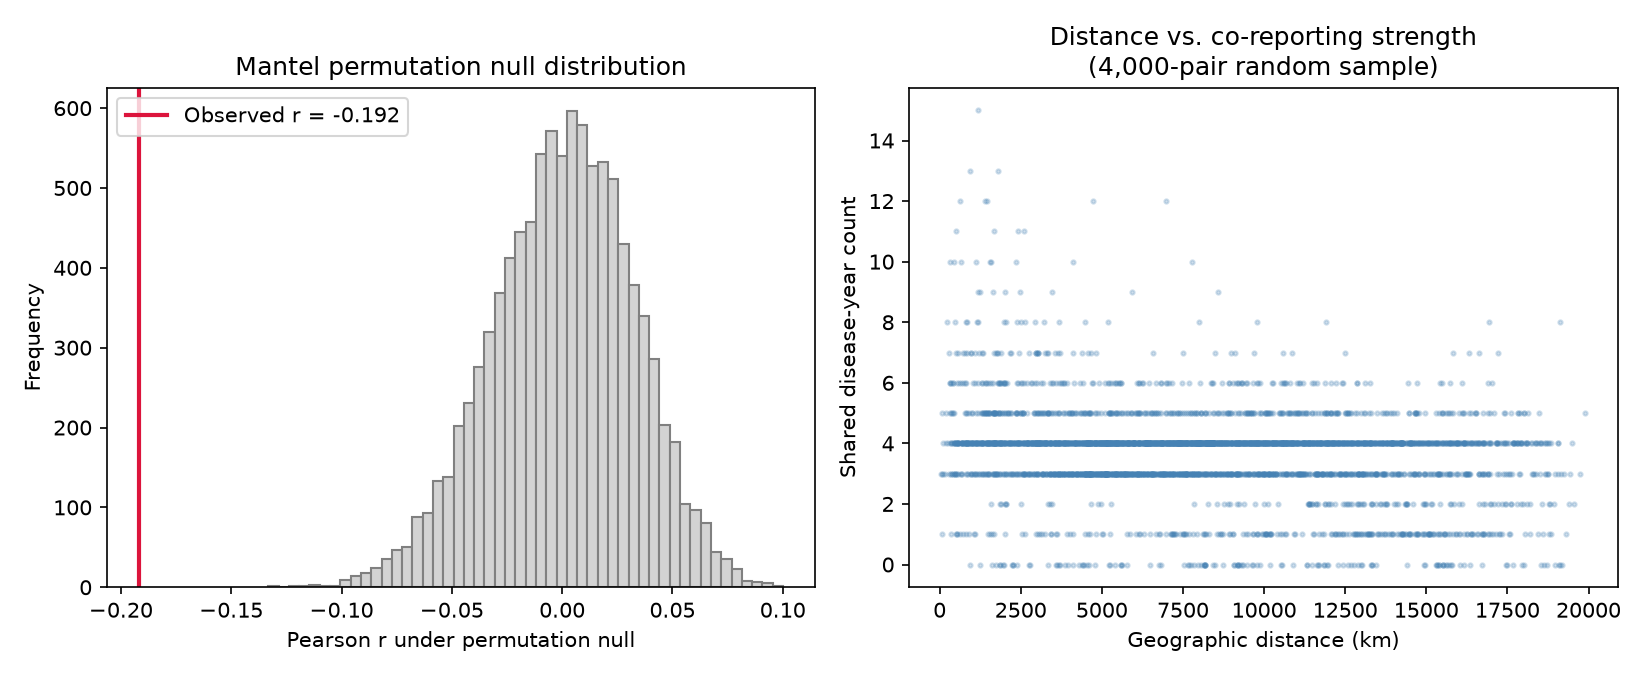
\includegraphics[width=0.85\linewidth]{figures/mantel_test_results.png}
\caption{Mantel permutation test results. Left: the observed correlation (red line) against
the null distribution generated by 9{,}999 label permutations. Right: a random sample of
4{,}000 country pairs showing the underlying relationship between distance and co-reporting
count.}
\label{fig:mantel}
\end{figure}

The effect size is modest: distance accounts for roughly four percent of the variance in
co-reporting strength by Pearson's $r^2$. A single globally reported disease such as
COVID-19 connects nearly every country regardless of distance, which dilutes any
distance-dependent signal coming from more geographically localized diseases. A dilution
account of this kind predicts that excluding the pandemic years should strengthen the
correlation. The data show the reverse: restricting the analysis to years before 2020
weakens the correlation ($r=-0.107$, $p<0.0001$). The timing of a country's COVID-19 report,
even though nearly every country eventually reported the disease, still followed the
geographic diffusion of the pandemic itself, so that neighboring countries reported in
closer temporal proximity to each other than distant countries did, strengthening the
distance signal during 2020--2022 rather than washing it out. This result depends on
comparing the statistical association across two overlapping but distinct time windows, and
motivates disaggregating the network by disease, taken up next, to clarify which diseases
drive the distance effect.

The statistical significance is unambiguous despite the modest effect size, converting the
qualitative impression from Fig.~\ref{fig:clustering-map} into a tested claim: geographic
distance has a small but statistically robust association with which countries co-report
infectious diseases.

\FloatBarrier

\subsection{Robustness to Travel Connectivity and Disease Transmission Mode}

The Mantel test above establishes that distance and co-reporting are correlated, but not
that distance does this explanatory work itself rather than standing in for travel
connectivity between well-connected countries. Applying the partial Mantel procedure from
Section~\ref{sec:methodology}, controlling for the air-travel connectivity matrix described
in Section~\ref{sec:connectivity-data}, the correlation between distance and co-reporting
weakens only slightly, from $r=-0.192$ unconditionally to a partial $r=-0.176$ ($p<0.001$
across 1{,}999 permutations). Distance and connectivity are themselves only weakly
correlated ($r=-0.105$): geographically close countries are somewhat, but not strongly, more
likely to have a direct flight route between them. Distance survives as a predictor of
co-reporting in its own right, not as a proxy for which countries happen to fly to each
other.

\begin{table}[H]
\centering
\caption{Partial Mantel Test Results, Controlling for Air-Travel Connectivity}
\label{tab:partial}
\begin{tabular}{lcccc}
\toprule
Stratum & Countries & Pairs & Partial $r$ & $p$ \\
\midrule
Full network & 233 & 26{,}203 & $-0.176$ & $<0.001$ \\
Vector-borne & 108 & 735 & $-0.070$ & $<0.001$ \\
Respiratory & 232 & 26{,}180 & $-0.144$ & $<0.001$ \\
Waterborne/food. & 105 & 1{,}402 & $-0.111$ & $<0.001$ \\
\bottomrule
\end{tabular}
\end{table}

Stratifying this confound-controlled test by transmission mode (Table~\ref{tab:partial})
produces a result that runs against the intuition that vector-borne diseases, being tied to
the geographic range of a mosquito, tick, or other arthropod vector, should show the
strongest distance effect of the three. Instead, vector-borne diseases show the weakest
distance-controlled correlation ($r=-0.070$), while respiratory diseases show the strongest
($r=-0.144$), with waterborne/foodborne diseases in between ($r=-0.111$).

This pattern is consistent with a distinction established in spatial ecology between two
sources of distance decay: decay driven by dispersal limitation, where similarity falls off
with distance because organisms, or in this case pathogens, cannot easily reach far-away
locations, and decay driven by environmental filtering, where similarity instead tracks an
environmental gradient that need not itself be spatially compact \cite{nekola1999}. Most
vector-borne diseases in this dataset, including malaria, dengue, and yellow fever, are
climatically constrained to the global tropical and subtropical belt, a habitat band that
circles the planet rather than occupying a single contiguous region; Brazil, Nigeria, and
Indonesia are all climatically suitable for these vectors while being geographically remote
from one another. Climate is a primary determinant of vector-borne disease distribution,
and that distribution is increasingly shaped by climate-driven range expansion independent
of simple geographic proximity \cite{paz2024}. If vector-borne co-reporting is governed
primarily by shared climate suitability rather than shared location, environmental
filtering by climate zone dilutes the distance-decay signal relative to diseases whose
spread depends more directly on regional contact and mobility patterns, such as respiratory
and waterborne/foodborne disease, which is the pattern observed here. Testing this mechanism
directly would require climate-zone data this analysis does not include, a natural target
for the future work discussed in Section~\ref{sec:limitations}.

\FloatBarrier

\section{Limitations and Future Work}
\label{sec:limitations}

The Mantel and partial Mantel tests above test the role of geographic distance directly
rather than asserting it, and the result holds after controlling for travel connectivity.
The structural limitation introduced in Section~\ref{sec:methodology}, that this network
connects countries rather than people, is not addressed by further statistical testing.
"Spread" at the country level means shared exposure to a reporting event, not a claim about
how a pathogen moved between two individuals. Additional confound control narrows which
alternative explanations remain plausible; it does not change what an edge in this network
represents. The results above should be read as a country-level surveillance and
pattern-detection signal, not a transmission-chain reconstruction.

Within that scope, narrower limitations remain. The dataset lacks node-level epidemiological
detail, case counts, severity, or case fatality, that would let centrality and clustering
results be weighted by health impact rather than by report count alone. Several
disease-specific subgraphs in Fig.~\ref{fig:subgraphs} and similar disease-year combinations
not shown form complete graphs among a small number of countries, which limits how much can
be inferred about transmission structure from those subgraphs individually. The air-travel
connectivity matrix counts route legs rather than passenger volume and leaves 1.6 percent of
routes unresolved to a country, and the disease transmission-mode classification leaves
thirteen diseases unclassified and a further fourteen in a labeled but heterogeneous "other
known route" category excluded from the stratified test.

Future work has two directions. The first stays within the current network: testing
additional candidate confounds, such as trade volume or shared official language, against
the partial Mantel framework already built here, and directly testing the climate-zone
explanation proposed above for the weak vector-borne distance effect, which this paper
proposes but does not verify. The second direction changes scope rather than extending the
current network: moving from country-level co-reporting to mobility-weighted or
genomic/phylogenetic transmission data would address the structural limitation above
directly, at the cost of either narrowing to a single well-sequenced pathogen or requiring
mobility data not available to this project.

\section{Conclusion}

This paper analyzed the global network of infectious disease co-reporting along temporal
and geospatial dimensions. The temporal analysis showed that network connectivity is highly
sensitive to globally synchronized events, rising sharply during the COVID-19 pandemic,
while remaining structurally distributed rather than concentrated around a small set of hub
countries, evidenced by a maximum k-core of 221 shared by most of the network. The
geospatial analysis showed that geographic proximity is associated with stronger disease
co-reporting connections, a relationship the Mantel permutation test confirms is
statistically significant and not an artifact of the network's dependency structure, that
survives controlling for air-travel connectivity in a partial Mantel test, and that holds,
and strengthens, when the pandemic years are included. Stratifying the confound-controlled
test by transmission mode showed the distance effect is weakest for vector-borne disease
and strongest for respiratory disease, a pattern consistent with environmental filtering
across a global climate zone overriding simple geographic proximity, a mechanism this paper
proposes from established ecological theory but does not test directly within this dataset.
These results move the central claim motivating this study, that distance matters for
disease co-reporting patterns, from a visual observation to a tested and confound-checked
finding. The network constructed here remains a country-level reporting signal rather than
a person-to-person contact network, and testing additional confounds and verifying the
climate-zone mechanism directly are the most promising directions for future work.

\section*{Acknowledgment}

The author thanks Dr. Assefaw Gebremedhin for feedback on an earlier version of this
analysis, in particular for the observation that a country-level co-reporting network
differs structurally from the contact networks conventionally used to study disease
transmission, and that the patterns identified are subject to confounding by factors other
than geography. That feedback directly motivated the partial Mantel and transmission-mode
stratification developed in Sections~\ref{sec:methodology} and~\ref{sec:results}.

\section*{Code and Data Availability}

All code, data, and the statistical validation analysis supporting this paper are openly
archived with a permanent DOI at Zenodo: Oje, S.A. (2026). Analyzing the Network of Disease
Distribution by Country and Distance. Zenodo. \url{https://doi.org/10.5281/zenodo.[XXXXX]}. This
includes the network construction and visualization notebook, the plain and partial Mantel
test scripts, the air-travel connectivity construction script, and the disease
transmission-mode classification. Code is released under the MIT License; the paper and
figures are released under CC BY 4.0.

\begin{thebibliography}{99}

\bibitem{baker2022} R.~E.~Baker, A.~S.~Mahmud, I.~F.~Miller, M.~Rajeev, F.~Rasambainarivo,
B.~L.~Rice, S.~Takahashi \emph{et al.}, ``Infectious disease in an era of global change,''
\emph{Nature Reviews Microbiology}, vol.~20, no.~4, pp.~193--205, 2022.

\bibitem{barabasi2023} D.~L.~Barab\'{a}si, G.~Bianconi, E.~Bullmore, M.~Burgess, S.~Chung,
T.~Eliassi-Rad, D.~George \emph{et al.}, ``Neuroscience needs network science,'' \emph{Journal
of Neuroscience}, vol.~43, no.~34, pp.~5989--5995, 2023.

\bibitem{serban2020} M.~Serban, ``Exploring modularity in biological networks,''
\emph{Philosophical Transactions of the Royal Society B}, vol.~375, no.~1796, p.~20190316,
2020.

\bibitem{leme2020} D.~E.~D.~C.~Leme, E.~V.~D.~C.~Alves, V.~D.~C.~O.~Lemos, and A.~Fattori,
``Network analysis: a multivariate statistical approach for health science research,''
\emph{Geriatrics, Gerontology and Aging}, vol.~14, no.~1, pp.~43--51, 2020.

\bibitem{who2020} World Health Organization, ``The top 10 causes of death,'' 2020.
[Online]. Available: \url{https://www.who.int/news-room/fact-sheets/detail/the-top-10-causes-of-death}

\bibitem{balcan2009} D.~Balcan, V.~Colizza, B.~Gon\c{c}alves, H.~Hu, J.~J.~Ramasco, and
A.~Vespignani, ``Multiscale mobility networks and the spatial spreading of infectious
diseases,'' \emph{Proceedings of the National Academy of Sciences}, vol.~106, no.~51,
pp.~21484--21489, 2009.

\bibitem{paz2024} S.~Paz, ``Climate change: a driver of increasing vector-borne disease
transmission in non-endemic areas,'' \emph{PLOS Medicine}, vol.~21, no.~4, p.~e1004382,
2024.

\bibitem{torres2022} J.~A.~Torres Mungu\'{i}a, F.~C.~Badarau, L.~R.~D\'{i}az Pavez,
I.~Mart\'{i}nez-Zarzoso, and K.~M.~Wacker, ``A global dataset of pandemic- and
epidemic-prone disease outbreaks,'' \emph{Scientific Data}, vol.~9, no.~1, p.~683, 2022.

\bibitem{kim2021} K.~Kim, S.~Yoo, S.~Lee, D.~Lee, and K.~H.~Lee, ``Network analysis to
identify the risk of epidemic spreading,'' \emph{Applied Sciences}, vol.~11, no.~7, p.~2997,
2021.

\bibitem{montresor2012} A.~Montresor, F.~De Pellegrini, and D.~Miorandi, ``Distributed
k-core decomposition,'' \emph{IEEE Transactions on Parallel and Distributed Systems},
vol.~24, no.~2, pp.~288--300, 2012.

\bibitem{mantel1967} N.~Mantel, ``The detection of disease clustering and a generalized
regression approach,'' \emph{Cancer Research}, vol.~27, no.~2 Part 1, pp.~209--220, 1967.

\bibitem{smouse1986} P.~E.~Smouse, J.~C.~Long, and R.~R.~Sokal, ``Multiple regression and
correlation extensions of the Mantel test of matrix correspondence,'' \emph{Systematic
Zoology}, vol.~35, no.~4, pp.~627--632, 1986.

\bibitem{legendre2000} P.~Legendre, ``Comparison of permutation methods for the partial
correlation and partial Mantel tests,'' \emph{Journal of Statistical Computation and
Simulation}, vol.~67, no.~1, pp.~37--73, 2000.

\bibitem{metal3d2024} metal3d, ``Countries coordinates with longitude and latitude,'' 2024.
[Online]. Available: \url{https://gist.github.com/metal3d/5b925077e66194551df949de64e910f6}

\bibitem{haversine2024} Wikipedia contributors, ``Haversine formula,'' \emph{Wikipedia, The
Free Encyclopedia}, 2024. [Online]. Available:
\url{https://en.wikipedia.org/wiki/Haversine_formula}

\bibitem{mayer2011} T.~Mayer and S.~Zignago, ``Notes on CEPII's distances measures: the
GeoDist database,'' CEPII Working Paper, 2011.

\bibitem{openflights2024} OpenFlights, ``Airport, airline, and route data,'' 2024. [Online].
Available: \url{https://openflights.org/data.php}

\bibitem{nekola1999} J.~C.~Nekola and P.~S.~White, ``The distance decay of similarity in
biogeography and ecology,'' \emph{Journal of Biogeography}, vol.~26, no.~4, pp.~867--878,
1999.

\end{thebibliography}

\end{document}
